\chapter{評価}
\label{chap:evaluation}

我々が実装した End.AN.NF の性能を評価するために,3つの実験を行った.
本章では,3つの計測実験で得られた結果から,提案手法が実用上十分なスループット性能を持っているか,及び実用的なレイテンシに収まっているのかを確認するために Linux に実装されている既存のパケット転送メカニズムと比較し評価する.
このうち2つはスループットについて,もう1つはレイテンシについて焦点を当てたものである.
最初の実験では,パケットサイズに基づくスループットを計測し,2つ目の実験では,netfilter ベースのアプリケーションにおけるフィルタールール数を増加させた際のスループットの変化を評価した.
3つ目の実験では,異なるパケット転送メカニズムに関連するレイテンシを計測した.
また,計測用パケットの送信に利用したトラフィックジェネレータ,及び評価の際に考慮したレシーブサイドスケジューリングについても解説する.
\section{計測の概要と予想}
\label{sec:eval-prediction}
End.AN.NF の性能を,3つの転送メカニズムと比較する.
比較対象は,End,End.DT4 と H.Encaps の組み合わせ,及び IPv4 である.
IPv4 は Linux のパケットフォワーディング性能におけるベースラインとして参照する.
図~\ref*{fig:hooks}に示すように,End.AN.NF が動作する場合,受信パケットは End と比較して2倍の数のフックポイントを通過する.
したがって,End.AN.NF の性能は End に劣ることが予想される.
一方で,End.AN.NF の性能は End.DT4 と H.Encaps の組み合わせよりも高いと予想される.
SRv6 でカプセル化されたパケットに netfilter のルールを適用する場合,バニラ Linux カーネルでの実用的なアプローチは End.DT4 と H.Encaps の組み合わせである.
しかし,バニラ Linux カーネルには SRv6 でカプセル化された状態の内部パケットに対して netfilter を適用する手法が実装されていない.
よって,パケットを一度カプセル化解除し,再度カプセル化する必要がある.
End.DT4 によってデカプセル化されたパケットは IPv4 パケットとして netfilter のフックポイントを通過し,H.Encaps は新しい SRH を格納する.
この方法では End.DT4 がパケットをデカプセル化し,その後 H.Encaps がパケットを再度カプセル化するため,オーバーヘッドが発生する.
したがって,このオーバーヘッドが性能の低下につながることが予想される.

3つの実験はすべて同じ構成,同じ環境で行った.
100Gbps のリンクで直結された2台のマシンを用意した.
2台のマシンは同一仕様で,CPU には Intel(R) Xeon(R) Silver 4310 12コア x2,メモリは 64GB DDR4-2666,NIC には Intel E810 100Gbps を搭載している.
CPU のハイパースレッディング機能は無効に設定した.
1台はトラフィック・ジェネレータとして,もう1台は SUT (System Under Test) として使用する.
トラフィック生成マシンには Ubuntu 22.04 と TRex~\cite{trex} をインストールし,テストトラフィックの生成に使用した.
一方,SUT マシンにはカスタマイズした Linux カーネル 5.15.106 をインストールし,End.AN.NF と,End.AN.NF の SID を設定するために独自に拡張した iproute2 コマンドを実装した.
また,2台のマシン間のリンクには2つの VLAN を設定し,テストトラフィックを送信するためのリンクと End.AN.NF 動作後に送信されるトラフィックが論理的に別のリンクになるようにした.


\section{TRex}
\label{sec:trex}
\textbf{[TRex について解説する]}

\section{レシーブサイドスケジューリング}
\label{sec:rss}
\textbf{[RSS について解説する]}

\section{パケットサイズ毎のスループット性能}
\label{sec:eval.thru-size}
End.AN.NF,End,IPv4,及び End.DT4 と H.Encaps の組み合わせについて,パケットサイズを増加させながらスループットを測定した.
この実験により,各パケット転送メカニズムにおけるパケットサイズによるスループットの変化が明らかになった.
この実験では,netfilter のルールは使用しなかった.
netfilter のフックポイントは通過するものの,実際に適用されるルールを何も定義せずに計測を行った.
End.AN.NF の,End に対するスループットの低下,及び End.DT4 と H.Encaps の組み合わせに対する性能の向上を評価した.

\subsection{計測内容}
\label{ssec:thru-size.summary}
トラフィック生成マシンで TRex によって生成されたトラフィックを,最小パケット長 126 バイトから最大パケット長 1518 バイトまでパケットサイズを変化させ,SUT マシンに送信した.
測定時のパケット長は次のように計算した: $l=174n+126$.
ここで $l$ はパケット長,$n$ は測定回数である.
$n=0$ から $n=10$ まで,合計10回の測定を行った.

最小パケット長として 126 バイトを選択した理由は,SID リストの長さが 2 である際のタグ付き VLAN を持つ UDP パケットの最小長が 126 バイトだからである.
End.AN.NF は,パケットの segleft をデクリメントするため,SID リスト長は少なくとも 2 である必要がある.
これは SID リストの長さが 1 の場合,segleft は 0 から始まり,End.AN.NF でデクリメントすると負の値になってしまうからである.
一方,End.DT4 は,segleft が 0 であることを必要とする.
End.DT4 は SRv6 ネットワークの終点で SRH をでカプセル化するビヘイビアである.
つまり,End.DT4 が動作するのは SID リストによって指定された最後のノードであるため,segleft はそれ以上デクリメントできない 0 である必要がある.
そこで,End.DT4 と H.Encaps の組み合わせの測定では,TRex は SID リスト長が 2 のパケットを生成し,segleft を 0 に設定した.
また,レシーブサイドスケジューリング (RSS) の仕組みを効果的に使用するため,TRex でパケットを生成する歳に内側の IPv4 パケットの宛先アドレスと送信元アドレスの両方をインクリメントした.
IPv4 パケットの計測の際は,SRv6 パケット長に合わせて UDP ペイロードにダミーデータを埋め込み,最小パケット長が 126 バイトから始まるようにした.
End.DT4 と H.Encaps の組み合わせの計測と同様,RSS を効果的に活用するため,パケット生成時に宛先アドレスと送信元アドレスをインクリメントした.
最大パケット長については,タグ付き VLAN ヘッダを含むイーサフレームの最大サイズが 1518 バイトであることから,今回の測定ではパケットサイズの上限を 1518 バイトに設定した.

\subsection{評価}
\label{ssec:thru-size.eval}
図~\ref{fig:size-thru} に,この実験の結果を示す.
End.AN.NF のスループットは,すべてのパケット長において End と比較して 6\% 以上の低下は見られない.
パケット長が 1518 バイトのとき,End.AN.NF は End と比べた際のスループットの低下が最も少なく,その低下は約 1.7\% である.
対して,パケット長が 478 バイトのとき,End と比較した際の End.AN.NF のスループットの低下は最も大きく,その低下は 約5.6\% である.
パケット長とスループットには相関がなく,大きな変動が見られた.
このスループットの低下は,End.AN.NF のパケットが End のパケットに比べて2倍の netfilter のフックポイントを通過することが原因として挙げられる.
ただし,そのスループット低下のレベルは許容範囲内に留まっている.

End.AN.NF のスループットを End.DT4 と H.Encaps の組み合わせと比較した場合,End.AN.NF は予想通り,パケット長に関係なく一貫して優れた性能を示している.
具体的には,End.AN.NF は End.DT4 と H.Encaps の組み合わせよりも,最大で 26.7\% 高いスループットを達成している.
グラフから,End.AN.NF と End.DT4 と H.Encaps の組み合わせとの間のスループットの差はパケット長の影響を受けていることが読み取れる.
短いパケットでは相対的な性能格差が大きくなり,長いパケットではその差は縮まる.
パケットサイズが小さくなるにつれて,1秒あたりのパケット転送レート (pps) は増加する.
結果として,パケットサイズが小さいほど,パケット転送のオーバーヘッドが顕著になる.

\begin{figure}[t]
    \centering
    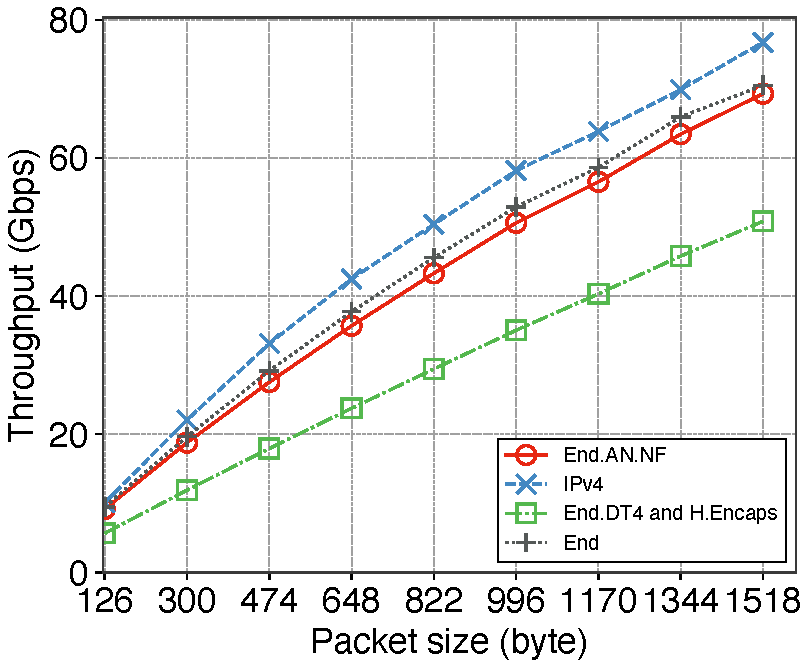
\includegraphics[width=0.95\linewidth]{img/size-throughput.pdf}
    \caption{Throughput per SRv6 End behaviors and IPv4}
    \label{fig:size-thru}
\end{figure}


\section{netfilter にインストールされたルール毎のスループット}
\label{sec:eval.thru-chains}
次に,End.AN.NF,IPv4,および End.DT4 と H.Encaps の組み合わせについて,netfilter にインストールするフィルタールールの数を変更しながらスループットを測定した.
フィルタールールのインストールには,netfilter ベースのアプリケーションとして nftables を使用した.
nftables では,ルールはチェインの集合として表現され,チェインにはベースチェインとレギュラーチェインの2種類がある.
nftables は,他のチェインがレギュラーチェインを参照している場合のみ,レギュラーチェインを使用する.
実験では,チェインの種類ごとにカウントを増やしながらスループットを測定した.
パケット転送メカニズムに関わらず,フィルタールールの追加によりスループットが低下することが予想される.
この実験は,フィルタールールによる各パケット転送メカニズムのスループット低下の特徴を明らかにすることを目的とする.

\subsection{nftables}
\label{ssec:thru-chains.nftables}
\textbf{[nftables について解説する. 特に regular chain と base chain について詳しく記す.]}


\subsection{計測内容}
\label{ssec:thru-chains.summary}
トラフィック生成マシンで TRex が生成したトラフィックを SUT マシンに送信した.
この測定では,パケット長を一貫して 126 バイトに設定した.
パケット長を 126 バイトに設定した理由はセクション~\ref{ssec:thru-size.summary} で説明したものと同じで,SID リスト長が 2 の場合のタグ付き VLAN の UDP パケットの最小長が 126 バイトだからである.

\subsection{評価}
\label{ssec:thru-chains.eval}
図~\ref{fig:rule-thru}は,ベースチェインのルール毎のスループットを示している.
全てのチェインルールがベースチェインのみで構成されるこれらのチェインルールは,nftables のチェインルールの定義の中でも最も性能の出ないルール定義の1つである.
この測定では,netfilter のフォワードフックポイントにフィルタールールを設定した.
netfilter は 1 つのフックポイントに複数のルールを設置できる.
実験を通して,このフックポイントで適用される同一のカスケードルールの数を増加させた.
すべてのパケット転送メカニズムにおいて,スループットはルール数の増加と共に低下する.
ルール数が増加するにつれて,3 つのパケット転送メカニズムすべてのスループットは約 0.4 Mbps に収束する.
End.AN.NF と IPv4 のスループットを比較すると,スループット低下における顕著な特性の違いは見られず,End.AN.NF は IPv4 に対して大きく劣るスループット低下特性を示さない.
一貫して,End.AN.NF は End.DT4 と H.Encaps の組み合わせのスループットを上回る.
しかし,このスループットの差はルール数が増えるにつれて縮小し,128 ルールではわずか 9\% の差まで減少した.
よって,レギュラーチェインのルール数が増加するにつれて,End.AN.NF の End.DT4 と H.Encaps の組み合わせに対する優位性は低下すると言える.

図~\ref{fig:reg-thru}は,ベースチェインのルール数毎のスループットを示している.
注目すべき点は,ルール数を増加させてもスループットの低下が認めれず,かつ End.AN.NF が一貫して End.DT4 と H.Encaps の組み合わせを上回っていることである.
レギュラーチェインのフィルタールールは,ベースチェインで測定した際と同じ構成である.
通過するパケットをすべてアクセプトするルールが定義されており,一度受け入れるルールが適用されたあとも,事前に決めた回数同じ内容のルールが適用され続ける.
しかし,レギュラーチェインのみから成るこのようなルール構成では,定義されたレギュラーチェインが他のチェインから参照されていないため,実際にはルールがパケットへ適用されることはない.
その結果,パケットが netfilter のフックポイントを通過する際に実際に適用されるルールの数は変わらない.

\begin{figure}[t]
  \centering
  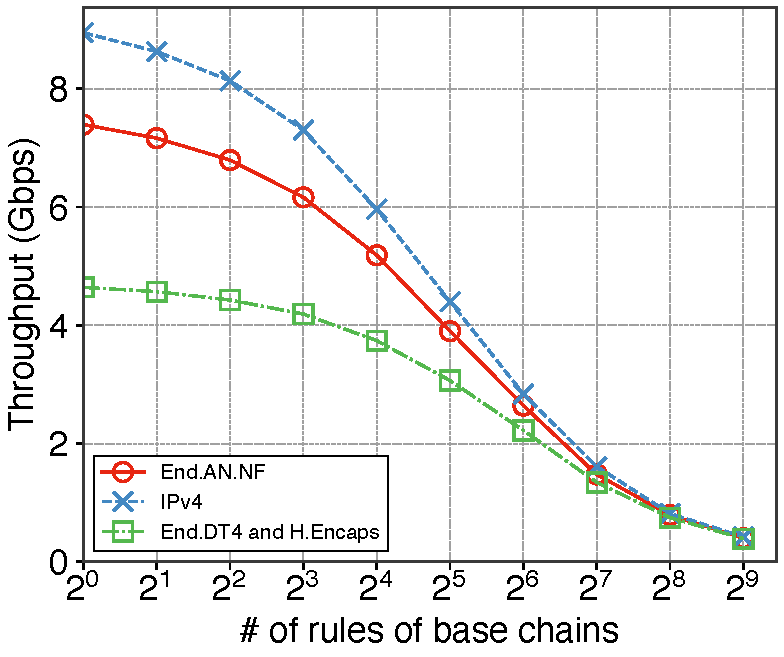
\includegraphics[width=0.95\linewidth]{img/rule-throughput.pdf}
  \caption{Throughput per number of rules of base chains}
  \label{fig:rule-thru}
\end{figure}

\begin{figure}[t]
  \centering
  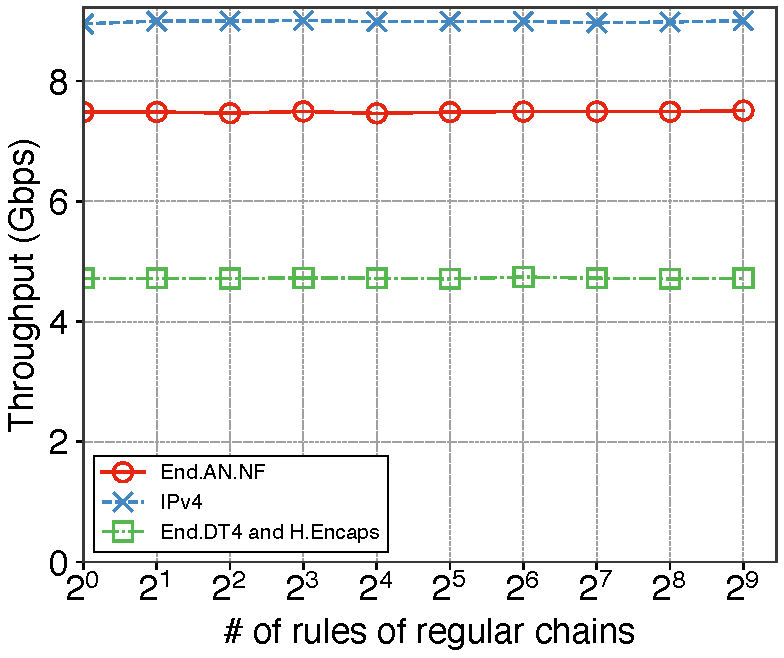
\includegraphics[width=0.95\linewidth]{img/regular-throughput.pdf}
  \caption{Throughput per number of rules of regular chains}
  \label{fig:reg-thru}
\end{figure}

\section{レイテンシ}
\label{sec:eval.rtt}
スループットと同様に End.AN.NF,End,IPv4,及び End.DT4 と H.Encaps の組み合わせについて,レイテンシを測定した.
この計測では特に,End.DT4 と H.Encaps の組み合わせと比較して,End.AN.NF のレイテンシがどれだけ改善されたのか評価することを目的としている.
この評価では,ベースラインとして IPv4 のレイテンシを用いた.

\subsection{計測内容}
\label{ssec:rtt.summary}
スループットと同様に,計測には TRex を使用し,パケット転送のレイテンシを測定した.
TRex はパケットの送受信時間間隔をマイクロ秒単位で測ることが可能である.
今回の測定は,パケット長を 142 バイトに設定した.
142 バイトの内訳について,先頭 126 バイトはセクション~\ref{ssec:thru-size.summary} で説明した通りで,End.AN.NF がの動作要件を満たす最小のパケットとして必要だからである.
追加の 16 バイトは,TRex がよるレイテンシを測定する際に利用するメタデータの埋め込みに使用される.
実験中,トラフィック生成マシンは SUT に対して毎秒 10000 個のパケットを10秒間送信した.
今回のレイテンシ測定では,RSS を無効化するために送信元アドレスと宛先アドレスを変更しなかった.
なぜなら,この規模の pps で RSS を使用してパケットを処理する CPU コアを分散させてしまうと,かえってレイテンシが悪化し,余分なジッタが発生することがあるからである.

\subsection{評価}
\label{ssec:rtt.eval}
計測結果を図\ref{fig:rtt} に示す.
これらのグラフの各データポイントは,100000 回のレイテンシ測定の平均値を表している.
End.AN.NF,End,IPv4 のレイテンシはどれも 16.0 マイクロ秒である.
対照的に,End.DT4 と H.Encaps の組み合わせは 19.0 マイクロ秒のレイテンシである.
マイクロ秒単位での測定では,End.AN.NF のレイテンシは End と IPv4 のレイテンシと一致し,End.DT4 と H.Encaps の組み合わせのレイテンシよりも約 15.8\% 高速であることが分かる.

\begin{figure}[t]
    \centering
    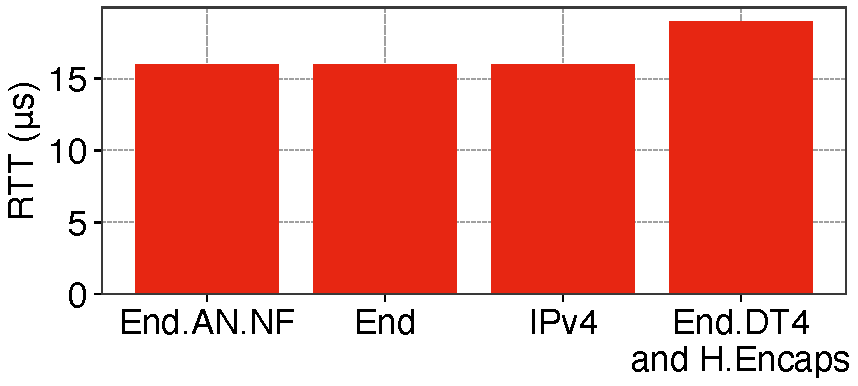
\includegraphics[width=0.95\linewidth]{img/latency.pdf}
    \caption{Latency per SRv6 End behaviors and IPv4}
    \label{fig:rtt}
\end{figure}